\chapter{Proper Time, Local Flatness, and Curvature from Parallel Transport}

The lecture announces two long-range goals, geodesics and their relation to gravity, but it begins somewhere else. Before we can speak sensibly about curved space-time, we need the space-time metric back on the table, together with proper time, the Minkowski signature, and the distinction between what a coordinate system calls time and what a clock actually records. From there the lecture turns to the question of flatness, shows how much of the metric can be simplified at a point, and only then returns to curves, geodesics, and parallel transport. Curvature finally appears not first as a tensor formula but as an obstruction: a vector transported around a closed loop fails to come back to itself.

\section{Space-Time Metric, Proper Time, and the Minkowski Signature}

For the first part of the lecture we are asked to think about space-time, not just space. The mathematics is the same in spirit as the mathematics of ordinary geometry, but the notation shifts. Instead of Latin indices \(m,n,\ldots\), Susskind begins with Greek indices \(\mu,\nu,\ldots\), running over \(0,1,2,3\), with \(0\) the time direction and \(1,2,3\) the spatial directions.

There is again a metric, and with it a notion of interval. In space-time that interval is written as proper time:
\begin{align}
d\tau^{2} &= g_{\mu\nu}\,dx^{\mu}dx^{\nu}, \\
\eta_{\mu\nu} &=
\begin{pmatrix}
1 & 0 & 0 & 0 \\
0 & -1 & 0 & 0 \\
0 & 0 & -1 & 0 \\
0 & 0 & 0 & -1
\end{pmatrix}.
\end{align}
In special relativity the metric is constant everywhere and is denoted by \(\eta_{\mu\nu}\). The lecture uses the signature \((+---)\): one plus sign for the time direction, and minus signs for the three spatial directions.

\begin{figure}[h]
\centering

\includegraphics[width=0.62\textwidth]{lecture_06_figure_02.png}
\caption{Minkowski metric and proper-time interval.}
\end{figure}

The last line on the board is slightly cramped, but the intended component form is clear from the lecture:
\begin{equation}
d\tau^{2} = dt^{2} - \frac{dx^{2}+dy^{2}+dz^{2}}{c^{2}}.
\end{equation}
If we use units in which \(c=1\), this becomes
\begin{equation}
d\tau^{2} = dt^{2} - dx^{2} - dy^{2} - dz^{2}.
\end{equation}
This is the space-time analogue of the distance formula. The displacement \(dx^{\mu}\) is the infinitesimal step along a worldline, and \(d\tau\) is the proper time along that worldline.

For slowly moving objects, the spatial term is negligible compared with the time term, and then \(d\tau\approx dt\). But once the motion is relativistic, the distinction matters: the interval along the trajectory is not the same thing as the coordinate time of an external frame.

\subsection{Question \& Answer}

\paragraph{Why does the moving clock record \(d\tau\) rather than \(dt\)?}

Because the clock moves with the object. It is not measuring the time coordinate of some external frame; it is measuring the interval along the worldline itself. The lecture makes the point with a geometric analogy: if we lay a tape measure along a curve in space, the tape does not record \(x\) or \(y\); it records distance along the curve. In the same spirit, a clock carried by the object is a kind of space-time tape measure. It marks off proper time along the trajectory. Coordinate time \(dt\) belongs to a chosen coordinate system; proper time \(d\tau\) belongs to the motion itself.

\section{Curved Coordinates Are Not Yet Curvature}

The lecture next makes a comparison that governs the rest of the chapter. General relativity stands to special relativity roughly as curved space stands to flat space. But one must be careful here. Curved coordinates are not yet the same thing as genuine curvature.

In flat space or flat space-time, one does not need curvilinear coordinates. In fact, if all we cared about were simple descriptions, introducing them would seem perverse. We do it because accelerated frames are physically important. In an inertial frame, free objects move on straight lines. In an accelerated frame, the same motions look curved, and the coordinate grid itself bends.

\begin{figure}[h]
\centering
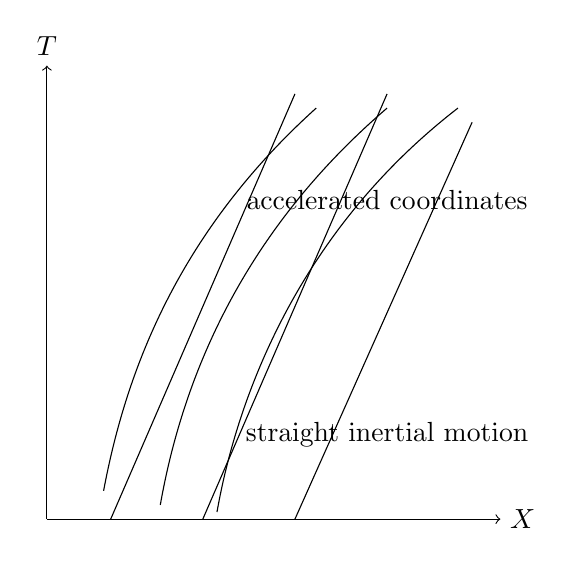
\begin{tikzpicture}[scale=0.9]
\draw[->] (0,0) -- (6.4,0) node[right] {$X$};
\draw[->] (0,0) -- (0,6.4) node[above] {$T$};

\draw (0.9,0) -- (3.5,6.0);
\draw (2.2,0) -- (4.8,6.0);
\draw (3.5,0) -- (6.0,5.6);

\draw (0.8,0.4) .. controls (1.1,2.0) and (1.8,4.0) .. (3.8,5.8);
\draw (1.6,0.2) .. controls (1.9,1.9) and (2.7,4.0) .. (4.8,5.8);
\draw (2.4,0.1) .. controls (2.7,1.8) and (3.6,4.1) .. (5.8,5.8);

\node at (4.8,4.5) {accelerated coordinates};
\node at (4.8,1.2) {straight inertial motion};
\end{tikzpicture}
\caption{Schematic inertial worldlines in \((T,X)\) and a curved coordinate grid adapted to an accelerated frame.}
\end{figure}

This is the old elevator story. A coordinate system adapted to an accelerating elevator can imitate a gravitational field. That is the content of the equivalence principle in its local form. But the lecture insists that we not stop there. A fake gravitational field produced by accelerated coordinates can be removed by going back to non-accelerated coordinates. A real gravitational field cannot be removed everywhere in this way.

A small freely falling elevator can eliminate gravity locally. Inside it, experiments look inertial. But only locally. If the elevator is large enough for the field to vary appreciably across it, tidal forces remain. One part of the elevator wants to fall differently from another. That is the obstruction. It is the first physical signal that we are not merely dealing with bad coordinates.

\section{What Does It Mean for Space or Space-Time to Be Flat?}

Once gravity has been recast as an obstruction problem, the lecture asks the mathematical version of the same question: what does it mean for a space, or a space-time, to be flat?

The first answer is global. A geometry is flat if one can find coordinates in which the metric is constant everywhere. In the simplest Euclidean case one can choose coordinates with
\[
g_{mn}=\delta_{mn},
\]
but the lecture immediately sharpens this: \(\delta_{mn}\) is not the essential point. One can also choose oblique but uniform coordinates, in which the metric is some other constant matrix. Flatness means constancy, not necessarily orthonormality.

Equivalently, one may say that flatness means the metric can be chosen so that all its first derivatives vanish everywhere:
\begin{equation}
\partial_{s}g_{mn}=0.
\end{equation}
This is already a three-index object: one derivative index together with the two symmetric metric indices.

The crucial turn comes next. Even before curvature has been defined in full generality, one can show that at a single point there is always enough coordinate freedom to make the first derivatives of the metric vanish there. That is the local mathematical counterpart of the freely falling elevator. We can always flatten the geometry at one point. What distinguishes true curvature is that this cannot, in general, be done everywhere at once.

There is also a distinction, emphasized later in the lecture, between bad coordinates and a genuinely bad geometry. Polar coordinates are singular at the origin, but the plane is not singular there; one simply changes coordinates. A real singularity is different. It is a place where no coordinate system makes the metric smooth. The cone tip will furnish the concrete example.

\section{Local Coordinate Freedom and Vanishing First Derivatives}

To see why the first derivatives of the metric can always be killed at a point, the lecture writes down a local coordinate transformation and counts freedoms against conditions. The argument is heuristic, but it is exactly the right heuristic.

Suppose we begin with coordinates \(x^{m}\) in which the metric is not locally constant at the chosen point. We introduce new coordinates \(y^{m}\), chosen to have the same origin, and expand:
\begin{equation}
y^{m}=x^{m}+c^{m}{}_{rs}\,x^{r}x^{s}+\cdots.
\end{equation}
The linear term has been taken to be the identity for convenience. The point of the argument lies in the quadratic correction. These coefficients \(c^{m}{}_{rs}\) are the knobs we turn in order to influence the first derivatives of the transformed metric.

\begin{figure}[h]
\centering

\includegraphics[width=0.62\textwidth]{lecture_06_figure_04.png}
\caption{Coordinate freedom and vanishing metric derivative.}
\end{figure}

The target condition is
\begin{equation}
\frac{\partial g_{mn}(y)}{\partial y^{s}}=0
\end{equation}
at the chosen point. Why might this be possible? Because the coefficients \(c^{m}{}_{rs}\) can be taken symmetric in \(r\) and \(s\):
\[
c^{m}{}_{rs}=c^{m}{}_{sr},
\]
since \(x^{r}x^{s}=x^{s}x^{r}\). For each fixed \(m\), this gives
\begin{equation}
\frac{D(D+1)}{2}
\end{equation}
independent coefficients, exactly the count written on the board.

\paragraph{Worked derivation.}
\begin{enumerate}
\item For fixed \(m\), the coefficients \(c^{m}{}_{rs}\) form a symmetric \(D\times D\) matrix in the indices \(r,s\).
\item A symmetric \(D\times D\) matrix has \(D(D+1)/2\) independent entries.
\item Since \(m\) itself runs over \(D\) values, the total number of adjustable coefficients is
\[
D\cdot \frac{D(D+1)}{2}=\frac{D^{2}(D+1)}{2}.
\]
\item The object \(\partial_{s}g_{mn}\) also has three indices, with \(m,n\) symmetric.
\item Therefore the number of first-derivative conditions matches the number of available quadratic coefficients.
\item The conclusion is that one can always choose the coordinates so that the first derivatives of the metric vanish at a single point.
\end{enumerate}

This is not a claim about second derivatives, third derivatives, and higher. The lecture is explicit here: once one goes to higher derivatives there are simply too many independent conditions. Local flattening extends through first order, not in general beyond.

\subsection{Question \& Answer}

\paragraph{Why is there enough coordinate freedom to kill the first derivatives, but not all higher derivatives?}

Because the quadratic part of the coordinate transformation has exactly the right number of independent coefficients to match the three-index object \(\partial_{s}g_{mn}\), where \(m,n\) are symmetric. That is a first-order statement. To eliminate second derivatives as well, one would have to control a much larger family of independent components, and the available higher-order coefficients do not suffice in general. So the lecture gives us a precise local theorem: first derivatives can always be removed at a point; higher derivatives encode genuine geometry.

\section{Christoffel Symbols and Metric Compatibility}

Once the first derivatives of the metric have been killed at a point, the next step is immediate. The Christoffel symbols are built from those first derivatives:
\begin{equation}
\Gamma^{r}{}_{mn}
=\frac{1}{2}g^{rs}\left(
\frac{\partial g_{sm}}{\partial x^{n}}
+\frac{\partial g_{sn}}{\partial x^{m}}
-\frac{\partial g_{mn}}{\partial x^{s}}
\right).
\end{equation}
So if at the chosen point
\begin{equation}
\frac{\partial g_{mn}(x)}{\partial x^{r}}=0,
\end{equation}
then at that same point
\begin{equation}
\Gamma^{r}{}_{mn}=0.
\end{equation}

\begin{figure}[h]
\centering

\includegraphics[width=0.62\textwidth]{lecture_06_figure_05.png}
\caption{Vanishing first derivatives and Christoffel symbols.}
\end{figure}

This already teaches an important lesson. Christoffel symbols cannot be tensors. A tensor that is nonzero somewhere cannot be made to vanish at a point merely by a coordinate transformation, but Christoffel symbols can. They reflect local coordinate effects as well as geometry.

The lecture then moves to the standard statement of metric compatibility:
\begin{equation}
\nabla_{r}g_{mn}=0.
\end{equation}
In components, for a rank-two covariant tensor, this is
\begin{equation}
\nabla_{r}g_{mn}
=
\partial_{r}g_{mn}
-\Gamma^{s}{}_{rm}g_{sn}
-\Gamma^{s}{}_{rn}g_{ms}.
\end{equation}
At the chosen point, in the locally flattened coordinates, both the ordinary derivative term and the Christoffel terms vanish, so \(\nabla g=0\) there. Since \(\nabla g\) is a tensor, if it vanishes in one coordinate system at a point, it vanishes in all coordinate systems at that point. And since the point was arbitrary, the standard conclusion is that \(\nabla g=0\) everywhere.

\subsection{Question \& Answer}

\paragraph{Is the argument for \(\nabla g=0\) circular?}

The lecture explicitly raises this objection, and it is worth preserving. The answer is: a little bit, yes. What is really being established is the consistency of the standard Levi-Civita construction. One assumes the usual form of covariant differentiation and the usual Christoffel symbols built from the metric, and then checks that with those definitions the metric is covariantly constant. Susskind does not present this as a pristine axiomatic proof; he presents it as the standard and consistent choice. That modesty should remain in the notes.

\section{Covariant Derivative Along a Curve, Geodesics, and Parallel Transport}

Only after this local groundwork is in place does the lecture return to curves. The starting point is the covariant derivative of a vector \(v^{m}\) along a curve \(x^{m}(s)\). If \(s\) is a parameter along the curve, then the tangent vector is
\[
\frac{dx^{p}}{ds}.
\]
The covariant derivative along the curve is
\begin{equation}
\frac{D v^{m}}{Ds}
=
\frac{dv^{m}}{ds}
+
\Gamma^{m}{}_{np}\,v^{n}\frac{dx^{p}}{ds}.
\end{equation}
The first term alone is not tensorial; the Christoffel term corrects for the fact that the coordinate basis itself may be varying as we move along the curve.

A geodesic is now recovered as the special case in which the vector being transported is the tangent vector itself. Set
\[
v^{m}=\frac{dx^{m}}{ds},
\]
and demand that it be parallel transported along the curve:
\begin{equation}
\frac{D}{Ds}\left(\frac{dx^{m}}{ds}\right)=0.
\end{equation}
This gives the coordinate geodesic equation
\begin{equation}
\frac{d^{2}x^{m}}{ds^{2}}
+
\Gamma^{m}{}_{np}\frac{dx^{n}}{ds}\frac{dx^{p}}{ds}
=0.
\end{equation}
That is the lecture's definition of the straightest possible curve in the space. In flat space, geodesics are straight lines. On a sphere they are great circles. In a general curved geometry they are the curves obtained by going incrementally straight ahead.

But the lecture immediately widens the scope. Parallel transport is not confined to tangent vectors and not confined to geodesics. We can choose any curve and any vector field defined along it, and say that the vector is parallel transported when its covariant derivative along the curve vanishes:
\begin{equation}
\frac{D v^{m}}{Ds}=0.
\end{equation}
Solving for the infinitesimal change in \(v^{m}\), one gets the update rule
\begin{equation}
dv^{m}=-\Gamma^{m}{}_{np}\,v^{n}\,dx^{p}.
\end{equation}
This is one of the important formulas of the lecture. It tells us how to move the vector from one infinitesimal step to the next so that it remains as constant as possible in the curved geometry. The differential \(dx^{p}\) here refers to the particular curve, so parallel transport is, from the start, path-dependent in its definition.

\paragraph{Worked update rule.}
\begin{enumerate}
\item Start from the condition \(D v^{m}/Ds=0\).
\item Expand the covariant derivative:
\[
\frac{dv^{m}}{ds}
+
\Gamma^{m}{}_{np}v^{n}\frac{dx^{p}}{ds}
=0.
\]
\item Multiply through by \(ds\).
\item Rearrange to obtain
\[
dv^{m}=-\Gamma^{m}{}_{np}\,v^{n}\,dx^{p}.
\]
\item Interpret this as the infinitesimal rule for advancing the vector along the curve.
\end{enumerate}

The lecture gives a physical picture as well. A gyroscope carried along a path, if not forcibly twisted, provides a concrete model of parallel transport. It preserves its direction as well as it can while being moved along the curve. If two vectors start perpendicular, and both are parallel transported, they remain perpendicular. In that sense parallel transport preserves the inner geometry of a little frame.

\subsection{Question \& Answer}

\paragraph{Does parallel transport mean keeping a fixed angle to the curve?}

No. This is one of the lecture's most useful corrections. If we transport a vector around an ordinary circle in flat space while keeping it parallel to itself, its angle relative to the tangent of the circle changes continuously. At one point it may be perpendicular to the tangent; later it may line up with it. What remains unchanged is not the angle with the curve, but the infinitesimal relation between the vector and its neighboring transported value.

There is, however, one important special case. In two dimensions, if the curve itself is a geodesic, then a parallel transported vector does keep a fixed angle with the tangent to that geodesic. The lecture mentions this only briefly and does not build a formal theory of torsion or higher-dimensional twisting here.

\section{Curvature as Path Dependence of Parallel Transport}

Now comes the main geometric idea. Once parallel transport has been defined, we can ask whether it gives a unique answer between two points. If we start with the same vector and transport it along two different curves joining the same endpoints, must we get the same final vector? The lecture immediately reformulates the question in a sharper way: transport the vector around a closed curve. Does it come back to itself?

In flat space, yes. In a curved space, not in general. This failure is the operational definition of curvature. A space is curved if there exist closed curves around which a parallel transported vector does not return to its original direction.

Before going to smooth surfaces, the lecture inserts an important distinction between coordinate singularities and real singularities. Polar coordinates are singular at the origin, but the plane is not. The bad behavior lies in the coordinates, not in the geometry. The tip of a cone is different. There is no coordinate system that makes the metric smooth there. That is a real singularity.

\begin{figure}[h]
\centering
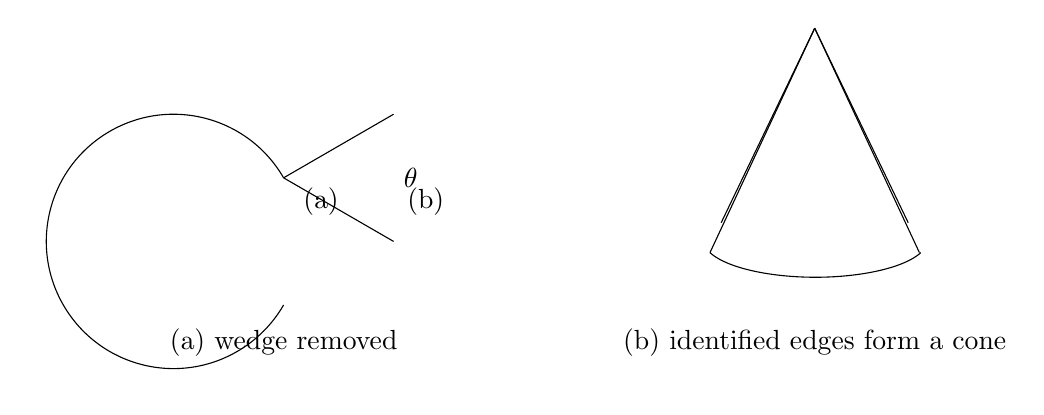
\begin{tikzpicture}[scale=0.95]
\draw (-4.2,0) -- (-4.2,0);
\draw (-4.2,0) node[below] {(a)};
\draw (-2.8,0) node[below] {(b)};

\draw (-4.6,0) -- (-4.6,0);

\draw (-4.0,0) -- (-4.0,0);

\draw (-5.5,0) -- (-5.5,0);

\draw (-4.8,0) -- (-4.8,0);

\draw (-5.8,0) -- (-5.8,0);

\draw (-4.5,0) -- (-4.5,0);

\draw (-5.5,0) -- (-5.5,0);

\draw (-5.0,0) -- (-5.0,0);

\draw (-5.2,0) -- (-5.2,0);

\draw (-5.6,0) -- (-5.6,0);

\draw (-4.2,0) -- (-4.2,0);

\draw (-5.2,0) -- (-5.2,0);

\draw (-5.0,0) -- (-5.0,0);

\draw (-5.4,0) -- (-5.4,0);

\draw (-5.6,0) -- (-5.6,0);

\draw (-5.2,0) -- (-5.2,0);

\draw (-5.0,0) -- (-5.0,0);

\draw (-5.4,0) -- (-5.4,0);

\draw (-5.8,0) -- (-5.8,0);

\draw (-5.0,0) -- (-5.0,0);

\draw (-5.6,0) -- (-5.6,0);

\draw (-5.0,0) -- (-5.0,0);

\draw (-5.6,0) -- (-5.6,0);

\draw (-5.3,0) -- (-5.3,0);

\draw (-5.0,0) -- (-5.0,0);

\draw (-5.8,0) -- (-5.8,0);

\draw (-5.2,0) -- (-5.2,0);

\draw (-5.8,0) -- (-5.8,0);

\draw (-5.4,0) -- (-5.4,0);

\draw (-5.6,0) -- (-5.6,0);

\draw (-5.0,0) -- (-5.0,0);

\draw (-5.2,0) -- (-5.2,0);

\draw (-5.4,0) -- (-5.4,0);

\draw (-5.8,0) -- (-5.8,0);

\draw (-5.2,0) -- (-5.2,0);

\draw (-6.2,0) -- (-6.2,0);

\draw (-5.0,0) -- (-5.0,0);

\draw (-5.8,0) -- (-5.8,0);

\draw (-6.0,0) -- (-6.0,0);

\draw (-5.4,0) -- (-5.4,0);

\draw (-6.2,0) -- (-6.2,0);

\draw (-6.4,0) -- (-6.4,0);

\draw (-6.0,0) -- (-6.0,0);

\draw (-6.6,0) -- (-6.6,0);

\draw (-6.0,0) -- (-6.0,0);

\draw (-6.6,0) -- (-6.6,0);

\draw (-5.8,0) -- (-5.8,0);

\draw (-6.8,0) -- (-6.8,0);

\draw (-5.8,0) -- (-5.8,0);

\draw (-5.0,0) -- (-5.0,0);

\draw (-6.4,0) -- (-6.4,0);

\draw (-5.0,0) -- (-5.0,0);

\draw (-6.6,0) -- (-6.6,0);

\draw (-6.1,0) -- (-6.1,0);

\draw (-6.3,0) -- (-6.3,0);

\draw (-6.7,0) -- (-6.7,0);

\draw (-6.0,0) -- (-6.0,0);

\draw (-5.9,0) -- (-5.9,0);

\draw (-6.6,0) -- (-6.6,0);

\draw (-5.9,0) -- (-5.9,0);

\draw (-6.7,0) -- (-6.7,0);

\draw (-6.0,0) -- (-6.0,0);

\draw (-6.6,0) -- (-6.6,0);

\draw (-6.3,0) -- (-6.3,0);

\draw (-6.7,0) -- (-6.7,0);

\draw (-6.1,0) -- (-6.1,0);

\draw (-6.4,0) -- (-6.4,0);

\draw (-6.8,0) -- (-6.8,0);

\draw (-6.2,0) -- (-6.2,0);

\draw (-6.9,0) -- (-6.9,0);

\draw (-6.2,0) -- (-6.2,0);

\draw (-4.7,0) arc[start angle=30,end angle=330,radius=1.7];
\draw (-4.7,0) -- (-3.23,0.85);
\draw (-4.7,0) -- (-3.23,-0.85);
\node at (-3.0,0.0) {$\theta$};
\node at (-4.7,-2.2) {(a) wedge removed};

\draw (2.4,2.0) -- (1.0,-1.0);
\draw (2.4,2.0) -- (3.8,-1.0);
\draw (1.0,-1.0) arc[start angle=200,end angle=340,x radius=1.5,y radius=0.5];
\draw (1.15,-0.6) -- (2.4,2.0);
\draw (3.65,-0.6) -- (2.4,2.0);
\node at (2.4,-2.2) {(b) identified edges form a cone};
\end{tikzpicture}
\caption{The cone as a flat sheet with an angular deficit and the corresponding identified surface.}
\end{figure}

The cone is the simplest model. Start with a flat sheet, cut out an angular wedge of size \(\theta\), and identify the cut edges. Away from the tip the geometry is flat. But the tip carries a genuine defect. Now test it with parallel transport.

\begin{figure}[h]
\centering
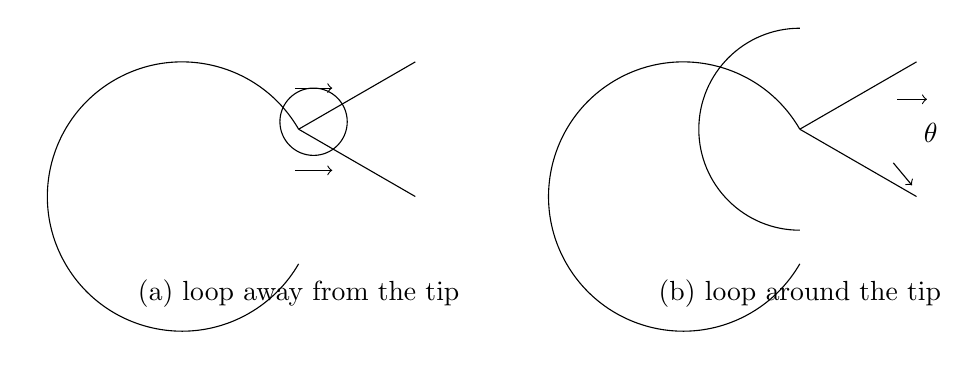
\begin{tikzpicture}[scale=0.95]
\draw (-4.5,0) arc[start angle=30,end angle=330,radius=1.8];
\draw (-4.5,0) -- (-2.94,0.9);
\draw (-4.5,0) -- (-2.94,-0.9);
\draw (-4.3,0.1) circle (0.45);
\draw[->] (-4.55,0.55) -- (-4.05,0.55);
\draw[->] (-4.55,-0.55) -- (-4.05,-0.55);
\node at (-4.5,-2.2) {(a) loop away from the tip};

\draw (2.2,0) arc[start angle=30,end angle=330,radius=1.8];
\draw (2.2,0) -- (3.76,0.9);
\draw (2.2,0) -- (3.76,-0.9);
\draw (2.2,1.35) arc[start angle=90,end angle=270,radius=1.35];
\draw[->] (3.50,0.40) -- (3.90,0.40);
\draw[->] (3.45,-0.45) -- (3.70,-0.75);
\node at (3.95,-0.05) {$\theta$};
\node at (2.2,-2.2) {(b) loop around the tip};
\end{tikzpicture}
\caption{A loop that avoids the cone tip returns a transported vector unchanged; a loop enclosing the tip returns it rotated by the angular deficit.}
\end{figure}

If the closed loop stays away from the tip, we can flatten that region onto the opened sheet and the vector returns to itself. But if the loop encloses the tip, the identification of the cut edges produces a mismatch. The vector comes back rotated by exactly the angular deficit:
\begin{equation}
\Delta\theta=\theta.
\end{equation}
This angle is independent of the detailed shape of the loop, provided the loop winds once around the tip. The cone therefore localizes curvature at a point.

The lecture then adds a subtle point. If we sand off the cone tip and replace the singular point by a smooth cap, a large loop around the same region still detects curvature inside it. The loop tells us that there is curvature in the interior, but not how that curvature is distributed. In the singular cone it is concentrated at a point. In the smoothed cone it is spread over a small region. Parallel transport diagnoses the presence of curvature before it gives the full local tensor description.

There is also a useful way to think about geodesics on the cone. In the opened wedge picture they are just straight lines. If a line crosses the cut, one simply re-open the cone elsewhere so that the same geodesic becomes a single straight segment on the new flat chart. This is exactly the lecture's cutting-and-pasting method.

The sphere supplies the smooth version of the same phenomenon. Take a small loop on a sphere. Locally, along that loop, the surface can be compared with a cone tangent to the sphere along the loop. A bug carrying a gyroscope around the loop cannot tell, from purely local measurements, whether it lives on the sphere or on the tangent cone. Therefore the transport defect is the same as on that cone.

\begin{figure}[h]
\centering
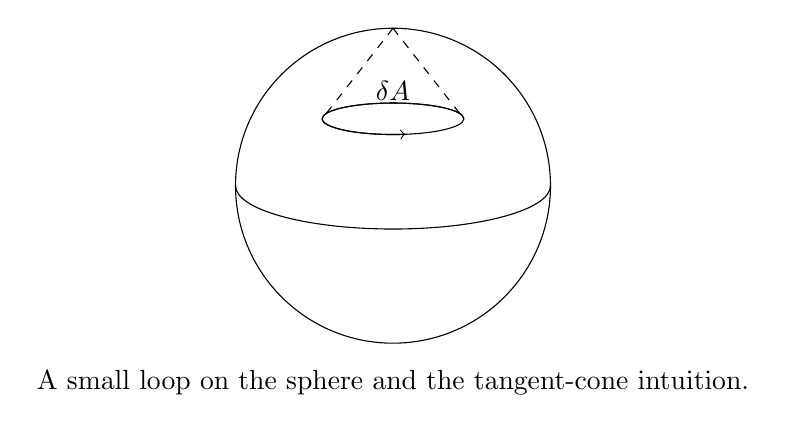
\begin{tikzpicture}[scale=1.0]
\draw (0,0) circle (2.0);
\draw (-2.0,0) arc[start angle=180,end angle=360,x radius=2.0,y radius=0.55];
\draw[dashed] (0,2.0) -- (-0.9,0.85);
\draw[dashed] (0,2.0) -- (0.9,0.85);
\draw (0,0.85) ellipse (0.9 and 0.2);
\draw[->] (0.9,0.85) arc[start angle=0,end angle=280,x radius=0.9,y radius=0.2];
\node at (0,1.2) {$\delta A$};
\node at (0,-2.5) {A small loop on the sphere and the tangent-cone intuition.};
\end{tikzpicture}
\caption{For a sufficiently small loop on a smooth surface, the transport defect is controlled by the enclosed area.}
\end{figure}

For small loops, the transport defect is small, and the lecture states the local two-dimensional law
\begin{equation}
\delta\theta \propto \delta A.
\end{equation}
More precisely, one defines the local curvature \(R\) by
\begin{equation}
\delta\theta = R\,\delta A
\end{equation}
for an infinitesimal loop. This is not yet the full curvature tensor of space-time. It is the two-dimensional local curvature law for a small region. It says that curvature measures the rate at which parallel transport around a tiny loop rotates a vector.

The sign of the curvature is fixed by orientation. Give the enclosed area a sign by the orientation of its boundary. If the vector rotates in the same sense as the positively oriented loop, the curvature is positive. If it rotates in the opposite sense, the curvature is negative. Symbolically, in the positive case,
\begin{equation}
\operatorname{sign}(\delta\theta)=\operatorname{sign}(\delta A).
\end{equation}
A sphere is positively curved. A saddle-shaped surface is negatively curved. The lecture describes negative curvature by an angle excess rather than an angle deficit: instead of cutting out a wedge and gluing the edges, one inserts an extra wedge. Transporting a vector counterclockwise around such a defect makes the vector rotate clockwise.

\paragraph{Side remarks.}
The Möbius strip appears as a useful but slightly misleading example. A vector taken around it can flip, but the surface is non-orientable and belongs to a different kind of discussion. The torus is more directly relevant. A torus described intrinsically as a rectangle with opposite sides identified can be flat. The familiar bagel-shaped torus embedded in three-dimensional space is not flat: its outer region is positively curved and its inner region negatively curved. These are instructive remarks, but the mathematical spine of the lecture remains the cone and the sphere.

At this point the lecture lifts everything back to space-time. The rules are the same. We still have a metric, Christoffel symbols constructed from it, and the same notion of parallel transport around closed curves. What changes is not the formalism but our ability to picture it. In space-time, curvature is the genuine gravitational field. Mass, or more generally energy and momentum, creates curvature. Particles then move on geodesics of the curved space-time, and in the appropriate limit those geodesics reproduce Newtonian motion with relativistic corrections.

\section{Summary}

The lecture begins by rebuilding the space-time interval and proper time, then uses gravity to motivate the distinction between curved coordinates and genuine curvature. Flatness means that the metric can be made constant, or equivalently that its first derivatives can be made to vanish, everywhere. At a single point this can always be done, and then the Christoffel symbols vanish there as well. From that local groundwork the lecture returns to curves: geodesics are curves whose tangent vectors are parallel transported, while parallel transport itself applies to any vector along any curve.

Curvature enters as path dependence. If a vector transported around a closed loop fails to return to itself, there is curvature inside the loop. The cone gives the sharpest example, the sphere gives the smooth one, and the small-loop law \(\delta\theta=R\,\delta A\) gives the local two-dimensional measure. The closing message is the one general relativity needs: space-time curvature is the real gravitational field, and geodesics are the relativistic replacement for Newtonian trajectories. The next lecture will turn that geometric idea into the curvature tensor itself.